\documentclass[
    a4paper,
    11pt,
    ]{scrreprt}
    
%\usepackage[textwidth=18cm,textheight=10cm]{geometry}

\usepackage[margin=3.cm]{geometry}

\usepackage{babel}
\usepackage[utf8]{inputenc}
\usepackage[T1]{fontenc}
\usepackage{lmodern}
\usepackage{amsmath}
\usepackage{amsfonts}
\usepackage{amssymb}
\usepackage{graphicx}
\usepackage{xcolor}

\usepackage[margin=0.5cm,font=small,format=plain,indention=0.25cm,labelfont=bf]{caption}

\usepackage{bm}

\usepackage{xhfill}
\definecolor{myblue}{rgb}{0.0, 0.40625, 0.675781}
\definecolor{myred}{rgb}{0.949219, 0.386719, 0.363281}
\definecolor{myviolet}{rgb}{0.257813, 0.1875, 0.246094}
\definecolor{myyellow}{rgb}{0.871094, 0.707031, 0.0273438}
\definecolor{mybrown}{rgb}{0.484375, 0.425781, 0.390625}
\definecolor{mybeige}{rgb}{0.957031, 0.863281, 0.753906}
\definecolor{mygray}{rgb}{0.632813, 0.640625, 0.632813}
\newcommand\sbullet[1][.5]{\mathbin{\vcenter{\hbox{\scalebox{#1}{$\bullet$}}}}}



\author{Lukas Manuel Rösel}
\title{Reservoir Computing Stuff}



\begin{document}

\maketitle

\tableofcontents

Hallo

\chapter{todo}

\section{things on the todo list.}

\subsection{programming work}

\subsection{research work}
\begin{itemize}
    \item check different weights
    \item check symmetry breaking nodes
    \item check "standard" topologies
    \item check breaking of standard topologies (extra links)
\end{itemize}

\subsection{graphics/plots}
\begin{itemize}
	\item stuart landau oscillator: complex plain, driven by input, with delayed feedback
	\item linear memory recall curve
    \item feed in plus system response for different ratios of theta and lambda
    \item rN from 1 to 32, rN from 1 to 32 with plot.
\end{itemize}

here comes the intro and all the important references...
small world \cite{WAT98}.

\subsection{theory}
	\begin{itemize}
		\item reservoir computing. definitions RC with delay, cc, masks, virtual nodes (more later)
		\item virtual networks through multiplexing. breakdown of analogy (random masks)
		\item tasks, training, covariance
		\item linear memory, legendre polynomials, narma
		\item linear regression. result: weights (plot weights for linear memories).
		\item networks
	\end{itemize}

\subsection{results}
	\begin{itemize}
		\item increasing network size
		\item increasing virtualization
		\item increasing input strength
	\end{itemize}

\chapter{one}

\section{Introduction}

	Reservoir Computing encompasses the field of machine learning in which the capacity to store and perform computations on data is investigated in a wide variety of dynamical systems (reservoirs). It can be understood as a generalization of earlier recurrent neural network architectures echo state networks (ESN) and liquid state machines (LSM). The name Reservoir Computing (RC) is particularly interesting as computations can be performed by the physical systems directly. Today "classical" computers of the van-Neumann-type (or more generally of the Turing-machine-type) need rely on the existence of a digital space in which everything is represented by a combination of discrete values ($0$ and $1$). To create such a virtual space the usual unpredictability that inhabits the scales in which modern computer circuits exist in has to be tamed in order to create this virtual computing space. As the scales of modern transistors shrink they rapidly approach the scales in which quantum effects become problematic. But even without quantum tunneling to worry about the production of transistors at tiny scales becomes increasingly difficult. The scales of modern silicone-transistor based cpus are so small adequate light sources needed to imprint the conduction paths are becoming rare and hideously expensive to operate. We are at the waning end of Moore's Law.
	
	Reservoir computing could circumvent several of today's difficulties by exploiting the physical dynamics directly without the need of discrete values of digital computation. 
	A wide variety of systems can be used e.g. a literal bucket of water can act as a reservoir that performs computations \cite{FER03}. Albeit the most interesting applications lie in potential optical computers. RC offers a way of utilizing the highly complex dynamics of optical systems in order to perform computation on them. Optical Computers in the form of lasers appear to be an ideal application of RC, because of the timescales that laser dynamics.  Optical reservoir computers already perform classification tasks on very timescales unmatched by modern silicon electronics \cite{BRU13a}
	Another expected benefit would be the vastly lower power consumption.  
	

	In recent years reservoir computing has received a lot of attention as bridge between machine learning and physics. As the end of "Moore's Law" is slowly encroaching we are in the waning years of an age of staggering performance leaps in silicon electronic circuits. Reservoir Computing as a way of utilizing the much smaller timescales at which optical systems operate offer a way of building drastically faster computers. There
	
	\cite{SAN17a} overview-paper

	\cite{LAR12} i fischer.
	
	\cite{ROE18a} paper von André. (has normalization?)
	
	\cite{JAE01} let's not train the networks.
	
	\cite{APP11} - original paper introducint the delay-based reservoir approach.
	
	\cite{ANT19} ? lesen!
	
	\cite{STE20} ? lesen
	
	\cite{ATI00} - NARMA10 task introduction.
	



\subsection{blabla}

Analyzing timeseries data is an important part of machine learning tasks. Many datasets can be regarded as a timeseries. Temperature, pressure and wind evolve over time and are fed into complicated climate prediction models in order to continue this timeseries into the future - predicting tomorrows weather patterns. The applications of extracting information from timeseries are vast. Predicting the stock market, driving an autonomous car based on a video stream and other vehicle metrics, recognizing types of heart arrhythmia or more general heart diseases and infections through analysis of electrocardiography by machine learning algorhithms (https://ieeexplore.ieee.org/abstract/document/7164783). Last, but not least: the most apparent machine learning application to date: voice recognition algorithms are predicting the meaning of audio information everytime we utter the magical words "Hi, Siri", "Ok, Google" or "Alexa...". 
It can also be argued that classical prediction tasks that do not involve time-conscious datasets like images fed into one directional feed forward networks 


\subsection{An analogy for reservoir computing}
	Let us imagine a pond. If we throw stones into the pond, they will make splashes and create concentric waves that propagate over the surface. If we miss the splash and therefor don't know the position of impact, could we still estimate where the stone landed two seconds prior? Could we estimate it three seconds prior? Or $20$ seconds prior? The answers would be yes, probably yes, possibly yes and our confidence would decrease further the longer we let the pattern of the waves progress. 
	So for short amounts of time the pond has some kind of "memory" about previous events. This memory will decay as the waves' amplitude gets smaller. The pond has some kind of fading memory.
	Additionally throwing similar stones at comparably similar positions of the pond will create similar wave patterns. The response of the pond to the stone's impact is not random. 
	From the pattern of waves other parameters might be extracted as well provided we have seen enough throws of stones with the corresponding wave patterns. 
	We might estimate size or weight, velocity, spin, angle and even shape of the stone just by looking at the waves. 
	
	Another counterintuitive possibility is the extraction of information that was \textit{not} inserted via the stones. For example given we might extract the product of the weights of two consecutive thrown stones by analyzing the interfering waves that originated at each of the impact regions. 
	
	
	

To understand the idea of reservoir computing one can imaging a pond of water. Now a stone is thrown into, creating ripples that propagate over the surface, reflect along edges and interfere with one another. The pond has some kind of short memory as ripples take time in order to disappear. 
It is easy to imagine that from the pattern of ripples a spectator could estimate the position of a stone that was thrown in shortly before.  
\section{Theory}
	
	%order:
	%reservoir condition - fading memory etc.



	\subsection{Stuart-Landau-Oscillator}
	The Stuart-Landau oscillator is a dynamical system often used to model basic class 1 lasers. It can be written either as a single complex differential equation (\ref{eq:stuartlandauequation}) or a set of two equations written in polar coordinates (\ref{eq:stuartlandauequation_polar}). From the equation in polar coordinates easy to see that the equation has rotational symmetry as the radial differential equation does not change with the dynamical variable $\phi$.
	
	\begin{equation}	
		\dot{z} = (\lambda +  i \omega + \gamma |z|^2 ) \; z
		\label{eq:stuartlandauequation}		
	\end{equation}
	
	\begin{equation}
		\begin{split}
		\dot{r} & = \lambda r + \operatorname{Re} (\gamma) \; r^{3} \\
		\dot{\phi} &= i \omega + \operatorname{Im}(\gamma) \; r^{2} 
		\end{split}
		\label{eq:stuartlandauequation_polar}
	\end{equation}

	For the radial dynamical variable the Stuart-Landau oscillator has two fixed points where the derivative $\dot{r}$ vanishes $r = 0$ and $r = \sqrt{-\lambda /\operatorname{Re}(\gamma)}$ whose stability depends on $\lambda$ and $\operatorname{Re}(\gamma)$. For $\operatorname{Re}(\gamma) < 0 $ (supercritical case).
	

	\begin{figure}
		\centering
		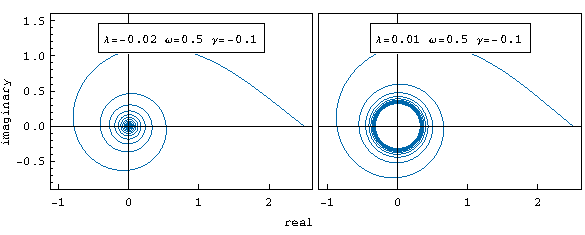
\includegraphics[width=0.99\linewidth]{pics/stuart_landau_complex_Focus_LC}
		\caption{$2$ very basic scenarios of the Stuart-Landau oscillator: Decay towards a single fixed point (left) or towards a limit cycle (right).}
		\label{fig:stuart_spiral}
		%nicht mehr
		%stuart_landau_basic.nb
	\end{figure}



The limit cycle (LC) which is shown in fig \ref{fig:stuart_spiral} is depending on the ratio or $\lambda$ and $Re \left[\gamma \right]$.





As can be seen in (eq. \ref{eq:stuartlandauequation}), the equation has a linear and a nonlinear term regarding the absolute value of $z$.

\subsection{Networks}

Vertices blabla \
Edges blabla. \

	\subsubsection{circulant Matrix}
    A circulant matrix has the same entries its row vectors, but with its entries rotated one element to the right relative to the previous row.
    
\subsection{virtual Nodes and multiplexing}
	here: papers for explanation! 
	\cite{KUR18}
	
	\cite{STE20} // off-resonance = better! --> reason for choosing 17 * 12.
	
	By multiplexing the input signal one can create virtual nodes in a network. The analogy to a real network can be best understood if the input signal is masked with a binary mask containing only values of either $0$ or $1$. 
	
	Different Mask types: discrete values with constant interpolation: binary, uniform - easy to implement)
	continuous: any function or repeating noise-patterns. (more difficult, but )
	
	
	here add dependency of total linear memory on number of nodes and virtal nodes.
	
	
	\begin{figure}
		\centering
		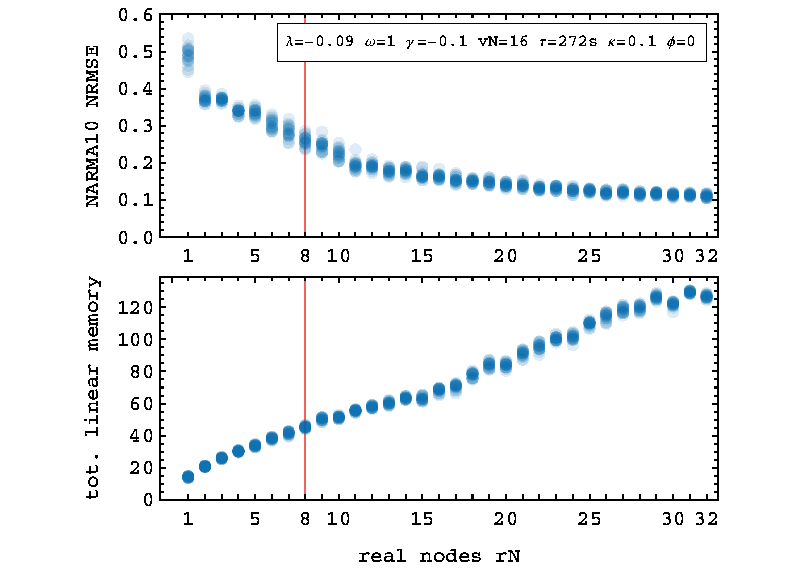
\includegraphics[width=0.9\linewidth]{pics/rNplot}
		\caption{changing rc performance for increasing number or real nodes $rN$ in unidirectianally coupled ring networks. (see some plot).}
		\label{fig:rN_1-32}
	\end{figure}

	\begin{figure}
	\centering
	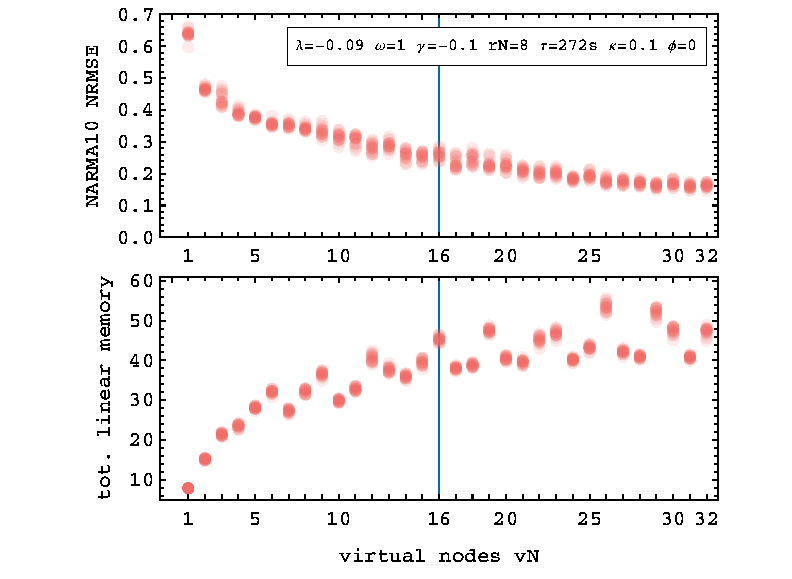
\includegraphics[width=15cm]{pics/vNplot}
	\caption{changing rc performance for increasing number or virtual nodes $rN$ in unidirectionally coupled ring networks. (see some plot).}
		\label{fig:vN_1-32}
	\end{figure}


\begin{figure}
	\centering
	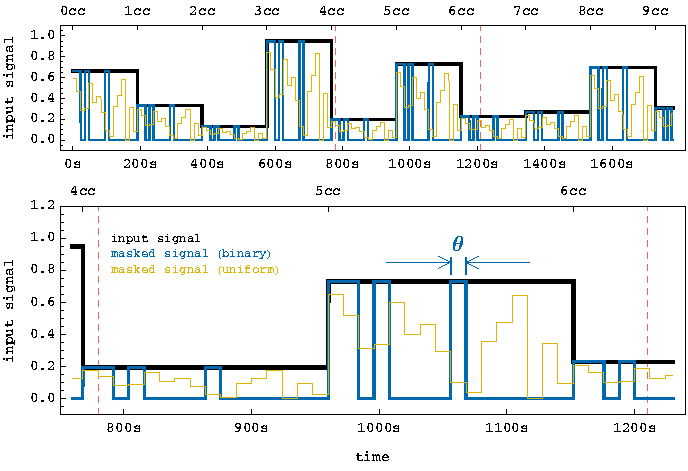
\includegraphics[width=15cm]{pics/signal_mask_vis}
	\caption{A timeseries (black) with constant interpolation ("sample \& hold") between samples and the corresponding masked signal (blue). The mask length is counted in clockcycles (cc) and the time per virtual node is counted in $\theta$. Here $\theta = 12s$ and $1cc = 16 \theta = 272s $}
	\label{fig:signal_mask_vis}
	%feedInVis_stuartlandau.nb
\end{figure}

	

\subsection{Dynamics of rings of stuart landau oscillators}
	pony-states (von André)
	
\subsection{Reservoir computing}
	
	\subsubsection{Measuring computation performance}
	We can measure how well a dynamical system perform computations by testing it in a variety of benchmarks. Dynamical systems are continuously evolving in time, thus reservoir computation mostly is mostly tested on timeseries data. There exist also approaches of using RC on datasets that do not involve datasets without a temporal dimension e.g. image classification of single images \cite{}
	
	
	
	
\subsection{Reservoir computing tasks}
	
	The reservoir computing performance of a given reservoir can be quantified by testing its predictions for certain tasks. The word "prediction" not necessarily means to predict the future value of something e.g. extend a timeseries into the future. Instead it often means the estimation of a value. A weather model which has been fed past temperature data can be tasked to "predict" the past humidity values. In machine learning the task is usually to predict a certain value or set of values from a set of inputs. Ideally the prediction can then be compared to the base truth and the difference between prediction and ground truth quantifies the error. The closer the prediction to the ground truth, the better the system performs a given task. 
	It is important to note that usually these predictions are not of singular values, but give a vector of probabilities. A neural network used for image classification will output a vector with values e.g. it is quantifying the "dog-ness", the "tree-ness" or the "car-ness" of an input image. The actual decision is made by choosing the entry with the highest probability. 
	For predictions based on timeseries data the same applies. They are represented by continuous values that the system puts out. Even if the desired output is of discrete nature e.g. "yes" or "no" the system will usually output a real number. 
	
	In general a sequence of inputs $u$ is drawn from a distribution. In this work only uniform distributions have been used. This sequence is used as input of a transformation which maps the sequence $u$ onto its target values $o$.

	
\subsubsection{Linear Memory Recall}
	The simplest task a reservoir can perform is to repeat the the information that was fed into it at a certain point in time.  

	\begin{figure}
	\centering
	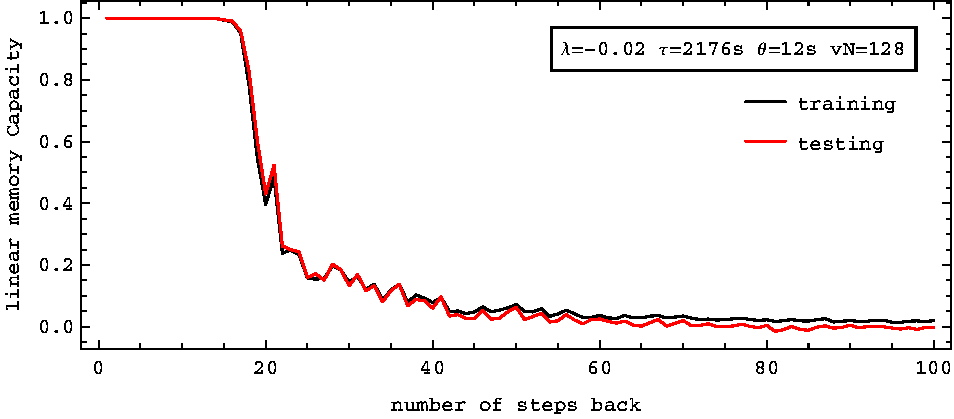
\includegraphics[width=0.99\linewidth]{pics/linearMemoryCurveN1}
	\caption{The linear memory capacities for differently many steps into the past. The system is able to perfectly reproduce inputs up until $12$ steps into the past. $N=1, vN=128, \lambda=-0.02, \omega=1, \gamma=-0.1, \theta=12, \tau=2176$. }
	\label{fig:linearMemoryRecallCurveN1}
	\end{figure}

	\begin{figure}
	\centering
	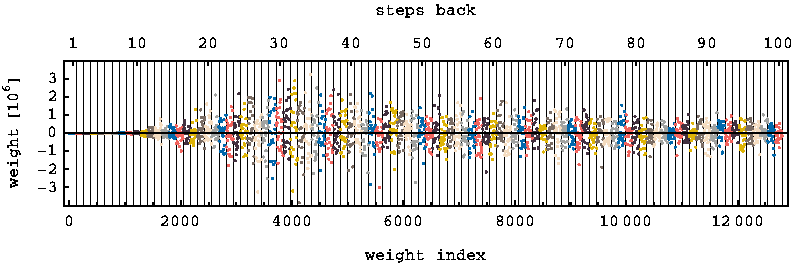
\includegraphics[width=0.99\linewidth]{pics/weight_plot}
	\caption{All weights $W_{i,s}$ attained through linear regression of the linear memory recalls $s \in [1,100]$ steps back. The system was a unidirectional ring with of $N_{real}=8$ and $N_{virtual}=16$ nodes. The total read-out dimension is $128$. For reconstruction of more recent inputs the inputs are small, but become enormous for inputs further in the past. This is the equivalent of "grasping at straws" as the system tries to extract information by multiplying microscopic fluctuations in the system state to linearily combine them to values between $[-1,1]$.}
	\label{fig:linearMemoryRecallWeights}
	\end{figure}

\subsection{Legendre polynomials as Nonlinear Transformations}
	In order to investigate the nonlinear transformation capabilities one can use Legendre Polynomials \ref{LegendrePolynomialsDegrees} in order to transform a given input into a system. Legendre Polynomials have the useful property of being orthonormal to every other polynomial within an interval $\left[-1,1\right]$. This makes them ideal in order to measure linearily independent nonlinear (but also linear) transformation capacities. Legendre polynomials $L_{d}(x)$ for degrees $d \in \{1-5\}$ are shown in fig.\ref{fig:legendreDegrees}). Depending on the definition they are scaled so that $L_{d}(1)=1$. The Legendre polynomial $L_{d}(x)$ is of course simply the identity. 
	The idea of measuring nonlinear (as well as linear) transformation capacities through the means of Legendre polynomials is largely inspired from the publication \cite{DAM12}. Hence the terminology used in the latter shall be used here as well. 
	As all nonlinear transformations of an input sequence $u^{h}$ can be expressed as a linear combination of Legendre polynomials with inputs in $u^{h}$ it is necessary to test all combinations. To elaborate: For the product of $2$ Legendre polynomials $L_{d_{1}}(u1)$ and $L_{d_{2}}(u2)$ with degrees $d_1$ and $d_2$ all combinations of $u1$ and $u2$ have to be calculated.
	
	Argh! kompliziert. \
	
	
	
	In order to investigate the different nonlinear transformation capabilities of a system it is necessary to iterate over all possible combinations of Products of Legendre polynomials  
	
	\begin{figure}
		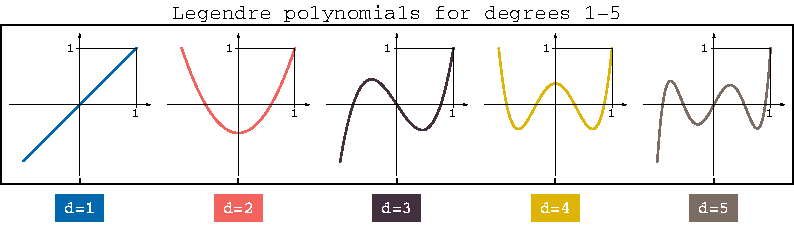
\includegraphics[width=0.99\linewidth]{pics/legendre_degrees}
		\caption{Legendre polynomials $L_{d}(x)$ for degrees $d \in \{1-5\}$ each shown for $x \in [-1,1]$ .}
		\label{fig:legendreDegrees}
	\end{figure}
	
	They are used in Neural networks as well blabla citecite findfind. 
	\cite{VOELKER Legendre Memory Units: Continuous-TimeRepresentation in Recurrent Neural Networks}
	%\begin{equation}
		
		
		
	%\label{eq:legendrePolynomials}
	%\end{equation}
	
	

\subsubsection{NARMA10 task}
	Lastly, the performance was investigated by measuring its capacity to compute the NARMA10 task. The Nonlinear Autoregressive Moving Average Task \cite{HER12} is used in many publications as a benchmark. The sequence is calculated using an average of its last $10$ steps while also being fed a product of a random sequence taken at two different positions. In order to perform well, systems need memory up to $10$ steps (hence the "10") into the past as well as nonlinear transformation capacities. Recently it has been shown that the task is not ideal as its difficulty depends non-trivially on the shape of the distribution used \cite{KUBOTA_Arxive}. \\
	The NARMA10 sequence is created by the iterative formula given by \ref{NARMA10equation}. It is fed $2$ inputs from a sequence $u$ which is drawn from a uniform distribution $U(0,0.5)$ on interval $\left[0,0.5\right]$.
	
	\begin{equation}
		A_{n+1} = 0.3 A_{n} + 0.05 A_{k}\left( \sum_{i=0}^{9} A_{k-9} \right) +1.5 u_{k-9} u_{k} + 0.1
		\label{NARMA10equation}
	\end{equation}


	%here schöne plots mit narma.
	

% different stuart landau scenarios - hopf bifurcation
\section{Results}

	\subsection{Highly symmetrical network topologies}
		\subsubsection{Ring networks}
		
		Rings with from N=1(edge case) to N=16
		Bidirectional Rings
		Bidirectional Rings with self-feedback and diffuse coupling
		
		\subsection{All to all coupled networks}
		N=3 - N=16 row normalization
		
	\subsection{Less symmetrical network topologies}
		\subsubsection{unidirectional rings with jumps}
			
		


\bibliographystyle{ag_label_wt}
\renewcommand{\em}{\itshape}
\renewcommand{\bf}{\textbf}
\bibliography{export}
\bibliography{ref}

\end{document}

